\documentclass[landscape]{article}
\usepackage{graphicx}
\usepackage[margin=0.5in]{geometry}
\DeclareGraphicsExtensions{.pdf}
\usepackage{nopageno}
\pagestyle{plain}
\usepackage{array}
\usepackage[export]{adjustbox}
\usepackage{booktabs}
\usepackage[abs]{overpic}
\usepackage{xstring,xifthen}
\usepackage{color}

\topmargin -1.2in

\parindent=0pt
\baselineskip=0pt
\parskip=0pt

% Participant Name
\def\yourname{Michael Pollan or longer name}

% Abundance Table
\def\abundTaxonA{Order NRP-J}
\def\abundSamplA{14.5}
\def\abundTaxonB{Genus \textit{Rickettsia}}
\def\abundSamplB{13.1}
\def\abundTaxonC{Genus \textit{Wolbachia}}
\def\abundSamplC{10.4}
\def\abundTaxonD{Order Sphingomonadales}
\def\abundSamplD{9.3}
\def\abundTaxonE{Family Erythrobacteraceae}
\def\abundSamplE{7.4}


% Enrichment Table
\def\enrichTaxonA{Genus \textit{SMB53}}
\def\enrichSamplA{7.4}
\def\enrichPopulA{0.4}
\def\enrichFolddA{20}
\def\enrichTaxonB{Family Peptostreptococcaceae}
\def\enrichSamplB{0.4}
\def\enrichPopulB{0.0}
\def\enrichFolddB{18}
\def\enrichTaxonC{Family Clostridiaceae}
\def\enrichSamplC{10.4}
\def\enrichPopulC{0.6}
\def\enrichFolddC{16}
\def\enrichTaxonD{Order Streptophyta}
\def\enrichSamplD{0.4}
\def\enrichPopulD{0.0}
\def\enrichFolddD{17}
\def\enrichTaxonE{Family Lactobacillaceae}
\def\enrichSamplE{3.3}
\def\enrichPopulE{0.0}
\def\enrichFolddE{70}


% Rare List
\def\rareList{This sample contained 11 rare and \textcolor{red}{1 unique} taxa, including the following: \textcolor{red}{Genus \textit{Candidatus Cardinium}}, Family Bifidobacteriaceae, Genus \textit{Wautersiella}, Genus \textit{Sphingobacterium}, Genus \textit{Christensenella}}


\usepackage{unicode-math}
\setmainfont[
   UprightFont = * Condensed Medium,
      BoldFont = * Medium,
    ItalicFont = * Condensed Medium,
%    ItalicFont = * Medium Italic,
]{Futura}



\begin{document}

\begin{tabular}{ @{} m{4.05cm} m{16cm} }
	
\includegraphics[height=0.08\textheight]{pdfs/logoshape.pdf} & 
\includegraphics[height=0.06\textheight]{pdfs/headerbw.pdf} \\
\end{tabular}
	
\vspace{0.65cm}

\begin{center}

\StrLen{\yourname}[\yournameLen]

\ifthenelse{\yournameLen < 28}{
	{\fontsize{40}{50}\selectfont {\MakeUppercase {\bf \yourname}}}
}{
	{\fontsize{36}{50}\selectfont {\MakeUppercase {\bf \yourname}}}
}

\end{center}

\vspace{0.65cm}

{\Huge What's in your American Gut?}

\vspace{2mm}

\begin{tabular*}{\textwidth}{ m{2.5in} m{1.3in} m{6.0in} }
    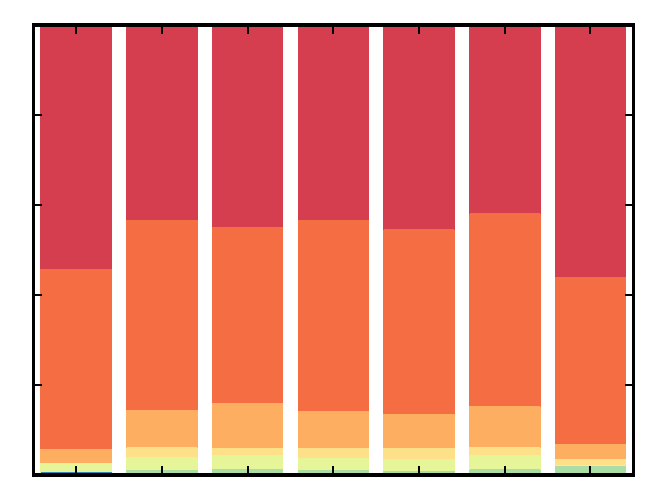
\includegraphics[width=2.5in]{pdfs/figure4.pdf} 
    &
    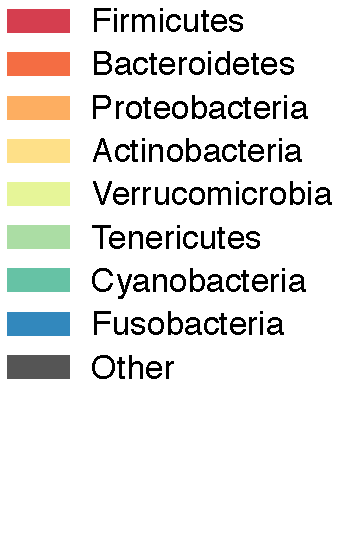
\includegraphics[width=1.3in]{pdfs/figure4_legend.pdf}
    &
    {\large 
    \vspace{-6mm}
    \parbox[b][][t]{6in}{
	\begin{tabular}{ c l r c l r r r }
    	    \multicolumn{3}{l}{\Large Your most abundant microbes:} & \multicolumn{5}{l}{\Large Your most enriched microbes:}\\ \addlinespace[2mm]
		\cline{2-3} \cline{5-8} \addlinespace[1mm]
		& Taxonomy & Sample & & Taxonomy & Sample & Population & Fold \\
		\cline{2-3} \cline{5-8} \addlinespace[1mm]
		& \abundTaxonA{} & \abundSamplA{}\% & & \enrichTaxonA{} & \enrichSamplA{}\% & \enrichPopulA{}\% & \enrichFolddA{}x \\
		& \abundTaxonB{} & \abundSamplB{}\% & & \enrichTaxonB{} & \enrichSamplB{}\% & \enrichPopulB{}\% & \enrichFolddB{}x \\
		& \abundTaxonC{} & \abundSamplC{}\% & & \enrichTaxonC{} & \enrichSamplC{}\% & \enrichPopulC{}\% & \enrichFolddC{}x \\
		& \abundTaxonD{} & \abundSamplD{}\% & & \enrichTaxonD{} & \enrichSamplD{}\% & \enrichPopulD{}\% & \enrichFolddD{}x \\
		\cline{2-3} \cline{5-8} \addlinespace[3mm]
		& \multicolumn{7}{p{5.2in}}{\large \rareList{}.}
	\end{tabular}
	}
	}
\end{tabular*}

\vspace{2mm}

{\Huge How do your gut microbes compare to others?}

\vspace{5mm}

\begin{tabular}{ l l l }

\begin{overpic}[height=0.30\textheight]{pdfs/figure1.pdf}
     \put(2,0){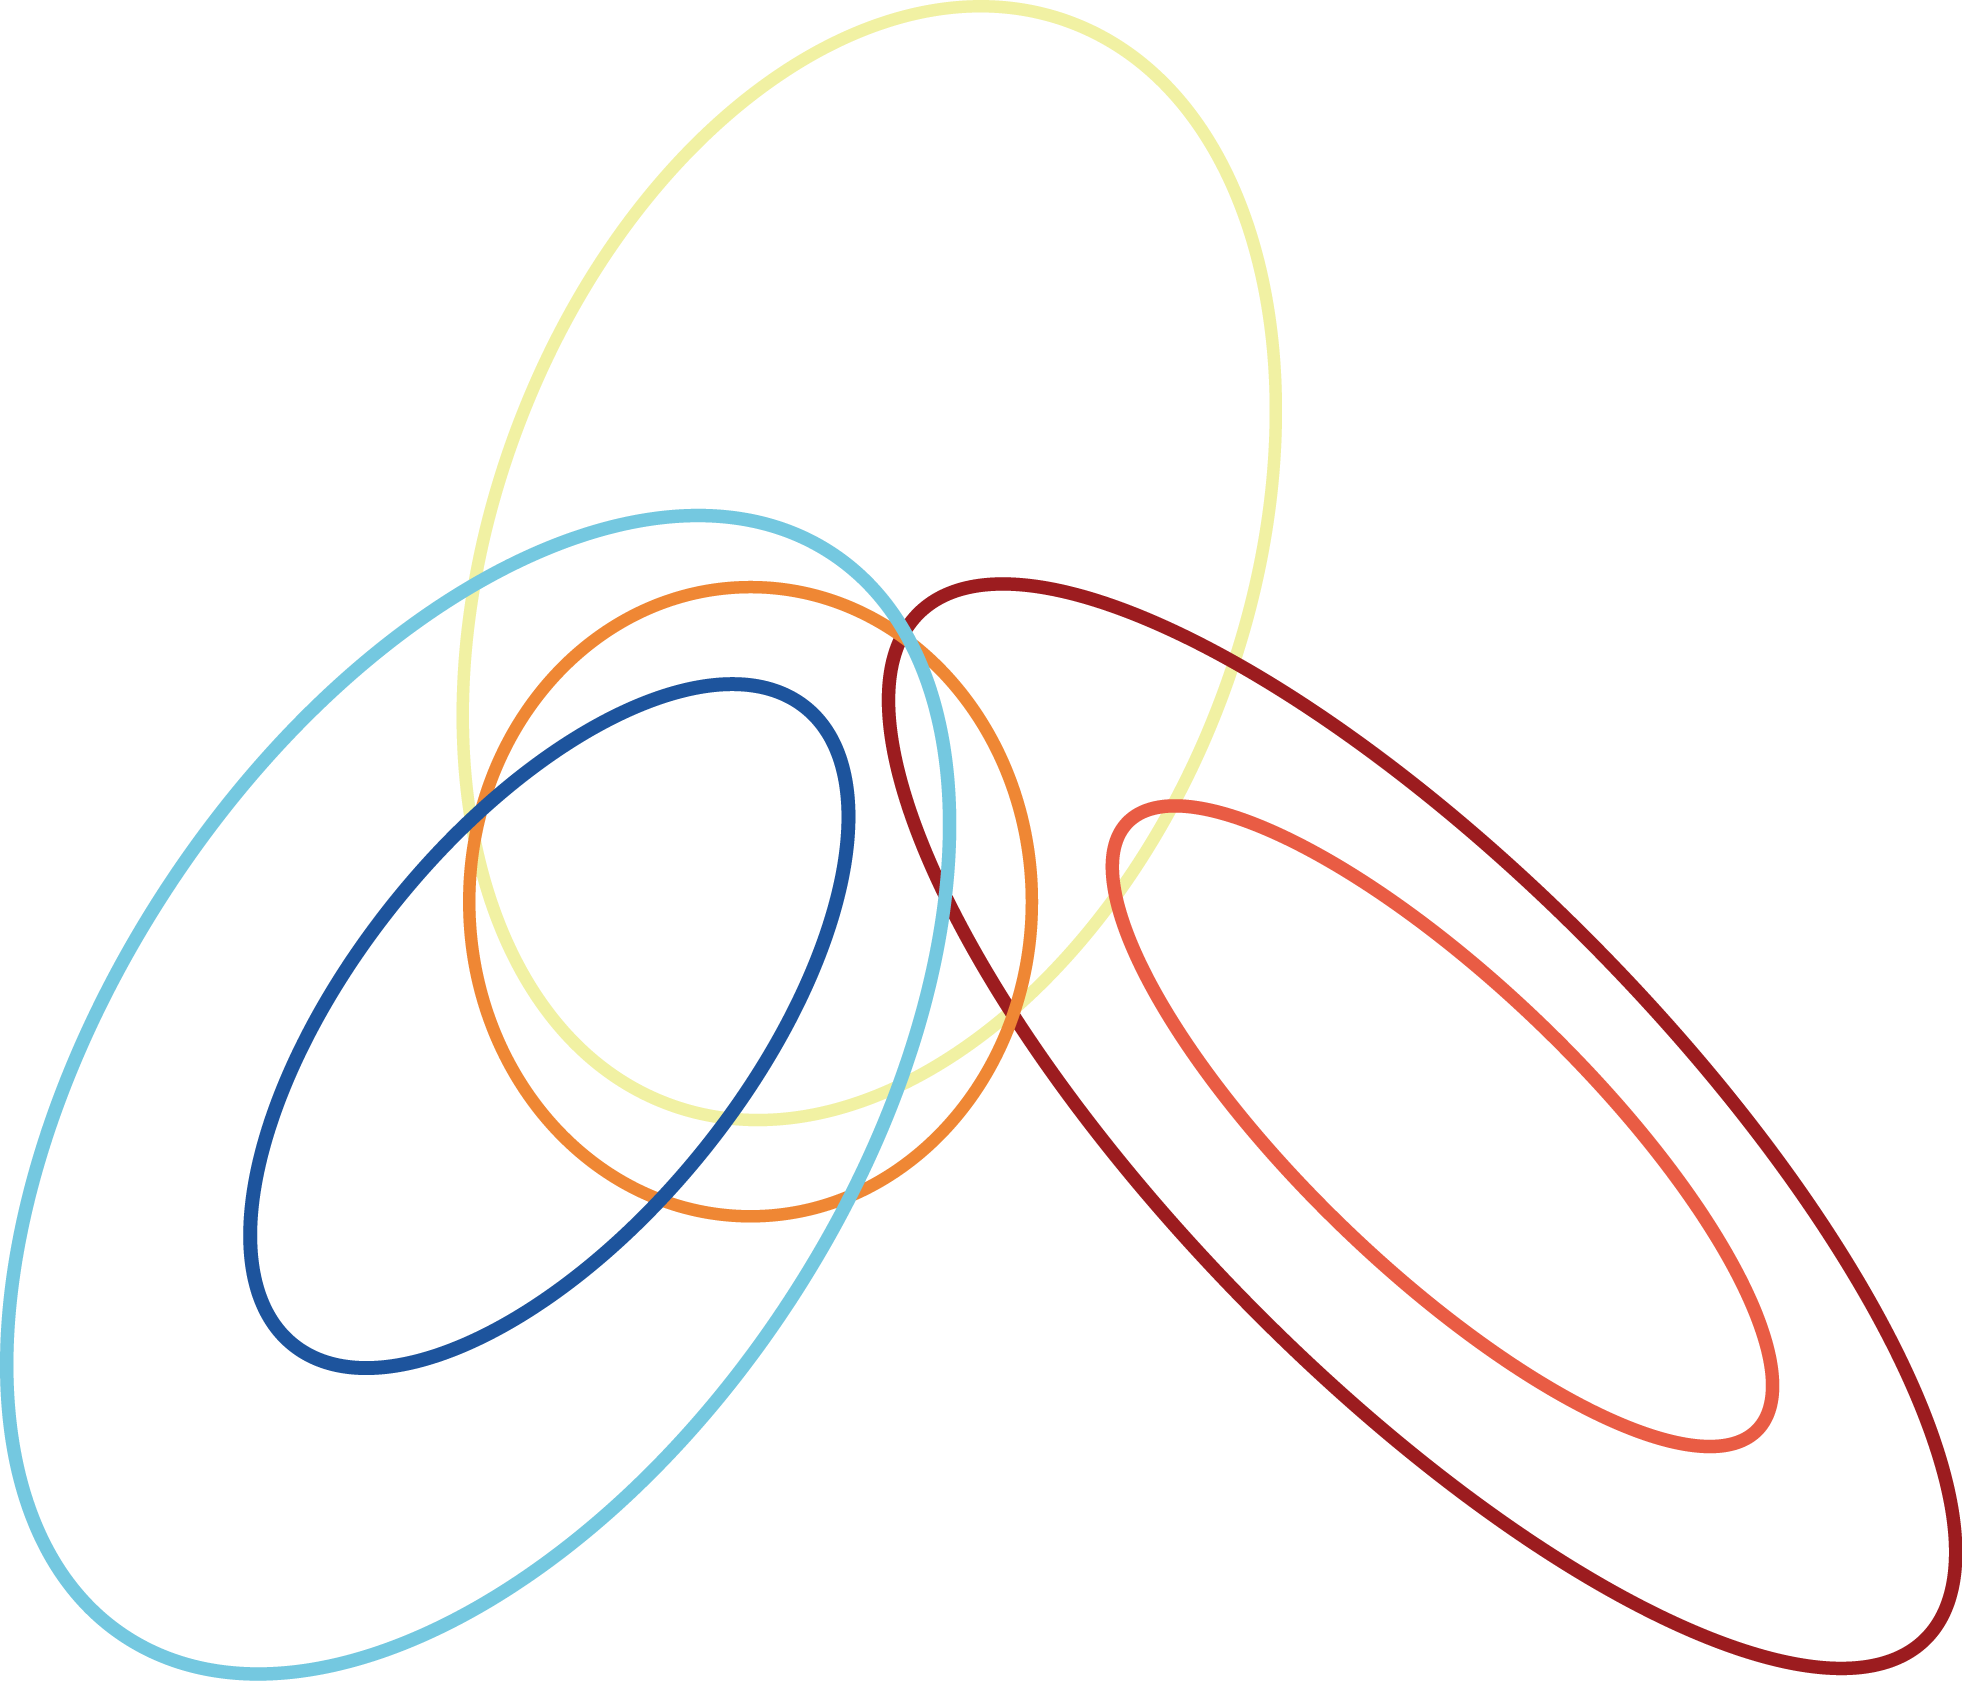
\includegraphics[scale=0.38]{pdfs/figure1_ovals.png}}
     \put(160,80){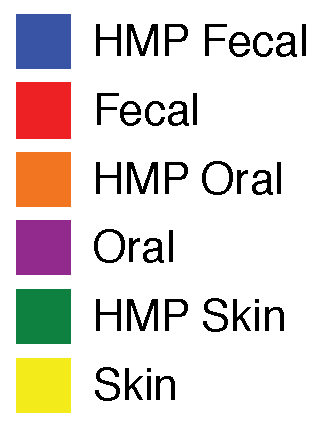
\includegraphics[scale=0.40]{pdfs/figure1_legend.pdf}}
\end{overpic}
&
\begin{overpic}[height=0.30\textheight]{pdfs/figure2.pdf}
     \put(200,15){
\includegraphics[scale=0.40]{pdfs/figure2_legend.png}}
\end{overpic}
&
\begin{overpic}[height=0.30\textheight]{pdfs/figure3.pdf}
     \put(200,15){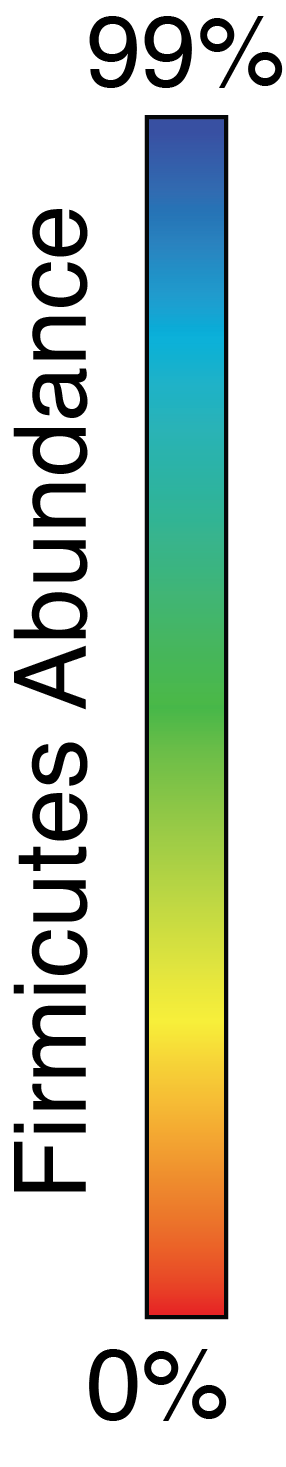
\includegraphics[scale=0.40]{pdfs/figure3_legend.png}}
\end{overpic}

\end{tabular}



\end{document}

